\documentclass{beamer}

\usepackage{xparse}
\usepackage{xfrac}
\usepackage[siunitx, american]{circuitikz}
\usepackage{hyperref}
\usepackage{cancel}
\usetikzlibrary{automata, arrows}

\newcommand{\R}{\mathbb{R}}

\NewDocumentCommand{\differential}{}{\mathrm d}

\NewDocumentCommand{\vocab}{m}{\textbf{#1}}


% Use this macro as follows:
%   d/dt => \ddt{}
%   dx/dt => \ddt{x}
%   df/dx => \ddt{f}[x]
%   d^2 f/d x^2 => \ddt[2]{f}[x]
%   \partial f/\partial x => \ddt[][\partial]{f}[x]
\NewDocumentCommand{\ddt}{s o  O{\differential} m O{t}}{
  \IfBooleanTF {#1}{%
    \IfNoValueTF{#2}{%
      \sfrac{#5 #4}{#5 #3}
    }{%
      \sfrac{#3^{#2} #4}{#3 #5^{#2}}
    }
  }{%
    \IfNoValueTF{#2}{%
      \frac{#3 #4}{#3 #5}
    }{%
      \frac{#3^{#2} #4}{#3 #5^{#2}}
    }
  }
}

\ExplSyntaxOn
\NewDocumentCommand{\mat}{ O{b} m }
 {
  \strategy_matlabmatrix:nn { #1 } { #2 }
 }

\seq_new:N \l_strategy_rows_seq
\seq_new:N \l_strategy_a_row_seq
\tl_new:N \l_strategy_matrix_tl

\cs_new_protected:Npn \strategy_matlabmatrix:nn #1 #2
 {
  \tl_clear:N \l_strategy_matrix_tl
  \seq_set_split:Nnn \l_strategy_rows_seq { ; } { #2 }
  \seq_map_inline:Nn \l_strategy_rows_seq
   {
    \seq_set_split:Nnn \l_strategy_a_row_seq { ~ } { ##1 }
    \tl_put_right:Nx \l_strategy_matrix_tl { \seq_use:Nn \l_strategy_a_row_seq { & } }
    \tl_put_right:Nn \l_strategy_matrix_tl { \\ }
   }
  \begin{#1matrix}
  \tl_use:N \l_strategy_matrix_tl
  \end{#1matrix}
 }
\ExplSyntaxOff

\usetheme{hutch-pdflatex}
% \renewcommand{\insertnavigation}[1]{}

\title{EE16B --- Midterm 1 Review}
\author{authors}
\institute{Presented by: }
\date{\today}

\begin{document}
    \section{}
	\begin{frame}
		\titlepage
	\end{frame}

	\begin{frame}{Disclaimer}
	This is an unofficial review session and HKN is not affiliated with this course. All of the topics we're reviewing will reflect the material you have covered, our experiences in EE16B, and past exams. We make no promise that what we cover will necessarily reflect the content of this midterm. While some course staff members may be among the presenters, this review session is still not official.
	\vspace{1em}
	
	This is licensed under the Creative Commons CC BY-SA: feel free to share and edit, as long as you credit us and keep the license. For more information, visit \\ \small{\url{https://creativecommons.org/licenses/by-sa/4.0/deed.en_US}}
	
	\end{frame}
	
	\section{CMOS Transistors and Logic}
	
	\begin{frame}{Transistors}
	    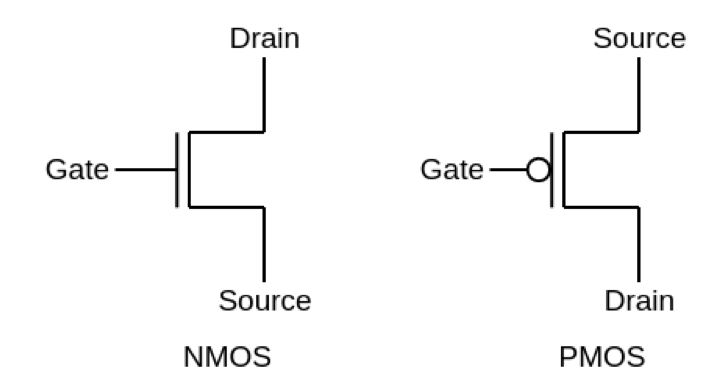
\includegraphics[width=0.5\textwidth]{mos.png}
	    
	    Two varieties of MOSFETs: P-type and N-type
	    \\
	    Any MOSFET has a characteristic threshold voltage $V_{th}$
	    \\
	    NMOS "turns on" (connects drain to source) when $V_{GS}>V_{th}$
	    \\
	    PMOS turns on when $V_{GS}<V_{th}$
	\end{frame}
	
	\begin{frame}{NMOS Logic}
	    We can build an inverter (a circuit that flips a 1 to a 0 and vice versa) with a single N-type MOSFET! \\
	    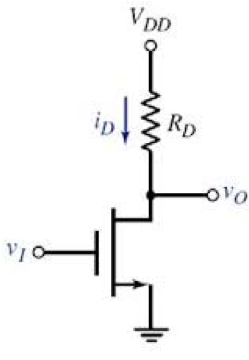
\includegraphics[width=0.2\textwidth]{nmos-inverter.png}
	    \\
	    What is $v_O$ when $v_I>V_{th}$? When $v_I<V_{th}$?
	    \\
	    Key disadvantage: what is the power dissipated when $v_I>V_{th}$? How can we rectify this?
	\end{frame}
	
	\begin{frame}{CMOS Logic}
	    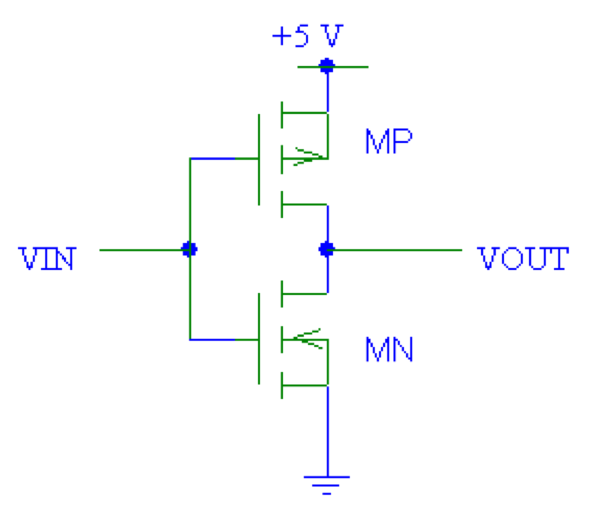
\includegraphics[width=0.4\textwidth]{cmos-inverter.png}
	    \\
	    Now, we have the same logical function as the NMOS inverter, but we're using more transistors and much less power is dissipated. Why?
	\end{frame}
	
	\begin{frame}{CMOS Logic}
	    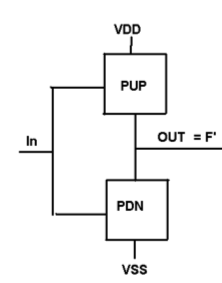
\includegraphics[width=0.3\textwidth]{cmos.png}
	    
	    This is broadly called Complementary Metal Oxide Semiconductor (CMOS) logic, using a Pull-Up Network of P-type and a Pull-Down Network of N-type MOSFETs.
	    \\
	    Now we can build circuits that perform logical functions out of MOSFETs!
	\end{frame}
	
	\begin{frame}{Transistors \& CMOS Wrap-up}
	    True or False:
	    \begin{enumerate}
	        \item Power (in the EE16B model) is dissipated in a CMOS circuit only when there is switching \\
	        \textbf{}
	        \item NMOS devices turn on with a large VGS and off with low VGS \\
	        \textbf{}
            \item For a given choice of inputs in a CMOS inverter circuit, we can create a low resistance path from ground to high voltage \\
            \textbf{}
	    \end{enumerate}
	\end{frame}
	
	\begin{frame}{Transistors \& CMOS Wrap-up}
	    True or False:
	    \begin{enumerate}
	        \item Power (in the EE16B model) is dissipated in a CMOS circuit only when there is switching \\
	        \textbf{True}
	        \item NMOS devices turn on with a large VGS and off with low VGS \\
	        \textbf{True}
            \item For a given choice of inputs in a CMOS inverter circuit, we can create a low resistance path from ground to high voltage \\
            \textbf{False}
	    \end{enumerate}
	\end{frame}
	
	\section{RC Circuits}
	
	\begin{frame}{RC Circuits}
    	The capacitor and resistor in a NOT circuit form the most basic RC circuit:
        
        Write down a differential equation describing the circuit below:

	    \begin{center}
	        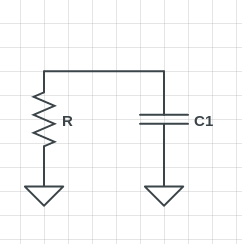
\includegraphics[width=0.5\textwidth]{rc-circuits-1.png}
	    \end{center}
	\end{frame}
	
	\begin{frame}{RC Circuits}
    	The capacitor and resistor in a NOT circuit form the most basic RC circuit:
        
        Write down a differential equation describing the circuit below:

	    \begin{center}
	        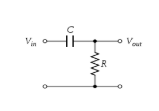
\includegraphics[width=0.5\textwidth]{rc-circuits-2.png}
	    \end{center}
	\end{frame}
	
	\begin{frame}{Solving the RC differential Equation}
    	Now that we have a differential equation describing the $V_{out}$, how do we actually solve it?
    	
    	$$\frac{dV_c}{dt} = -\frac{1}{RC}V_c$$
        
        We can think of the the differential operation as a linear operator that scales $V_c$, or an eigenfunction.

	    $$[\frac{d}{dt}]V_c = \lambda{V_c}$$
	\end{frame}
	
	\begin{frame}{Solving the RC differential Equation}
    	Which function is scaled by a constant when differentiated?
    	
    	$$Ae^{\lambda{t}}$$
    	
    	$$\frac{dV_c}{dt} = -\frac{1}{RC}V_c$$
    	
    	The solution to first order differential equations is:
    	
    	$$V_c(t) = V_c(0)e^{\frac{-t}{RC}}$$
	\end{frame}
	
	\begin{frame}{RC Differential Equation: Non-homogenous case}
	    How do you solve a RC circuit with a voltage source?
    	
    	\begin{center}
    	    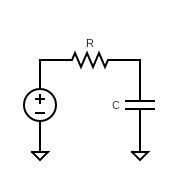
\includegraphics[width=0.2\textwidth]{rc-circuits-3.png}
    	\end{center}
    	
    	Applying KCL at the top right node, along with Ohm’s law and the capacitor relationship, we get:

        $$\frac{dV_c}{dt} = \frac{1}{VC}(V_s - V_c)$$
        
        We can't easily solve this equation, so we change variables to
        
        $$x = V_c - V_s$$
	\end{frame}
	
	\begin{frame}{RC Differential Equation: Non-homogenous case}
	    Now, we have $\frac{dx}{dt} = -\frac{x}{RC}$
    	
    	We already know how to solve this differential equation, and we get                              
        $$x(t) = x_0e^{-\frac{t}{RC}}$$
        
        Finally, change back to the original variables by substituting $V_c$ - $V_s$ for $x$
    	
    	$$V_c(t) = V_c(0)e^{-\frac{t}{RC}} + V_s(1 - e^{-\frac{t}{RC}})$$
	\end{frame}
	
	\begin{frame}{Change of Basis}
	    In the standard basis, we write vectors as a linear combination of the standard basis vectors.

        $$\vec{x} = \mat{x_1;x_2} = x_1\mat{1;0} + x_2\mat{0;1}$$
        
        Likewise, we can write our x vector as a linear combination of some other basis vectors. For example, if our V-basis has basis vectors $\vec{v_1}$ and $\vec{v_2}$:
        
        $$\vec{x} = \tilde{x_1}\cdot\vec{v_1} + \tilde{x_2}\cdot\vec{v_2} = V\vec{\tilde{x}}$$
        
        We can go from the V-basis to the standard basis by applying the V-matrix to x, and go from the standard basis to the V-basis by applying V-inverse
	\end{frame}
	
	\begin{frame}{Change of Basis Diagram}
    	\begin{columns}[onlytextwidth,T]
        	\column{\dimexpr\linewidth-40mm-5mm}
        	    \begin{itemize}
        	        \item When you are doing change of basis for systems of equations, it is useful to use a diagram mapping transformations between basis
                    
                    \item Given $T$, to find $T_a$ you would trace the path from $u_a$ to $v_a$, applying each transformation to the left of the previous:
                    
                    $A \implies TA \implies A^{-1}TA$
                    
                    $T_a = A^{-1}TA$
                    
                    \item Step by step, we have $Au_a = u \implies TAu_a = v \implies A^{-1}TAu_a = v_a$
        	    \end{itemize}
    	    
    	    \column{40mm}
    	        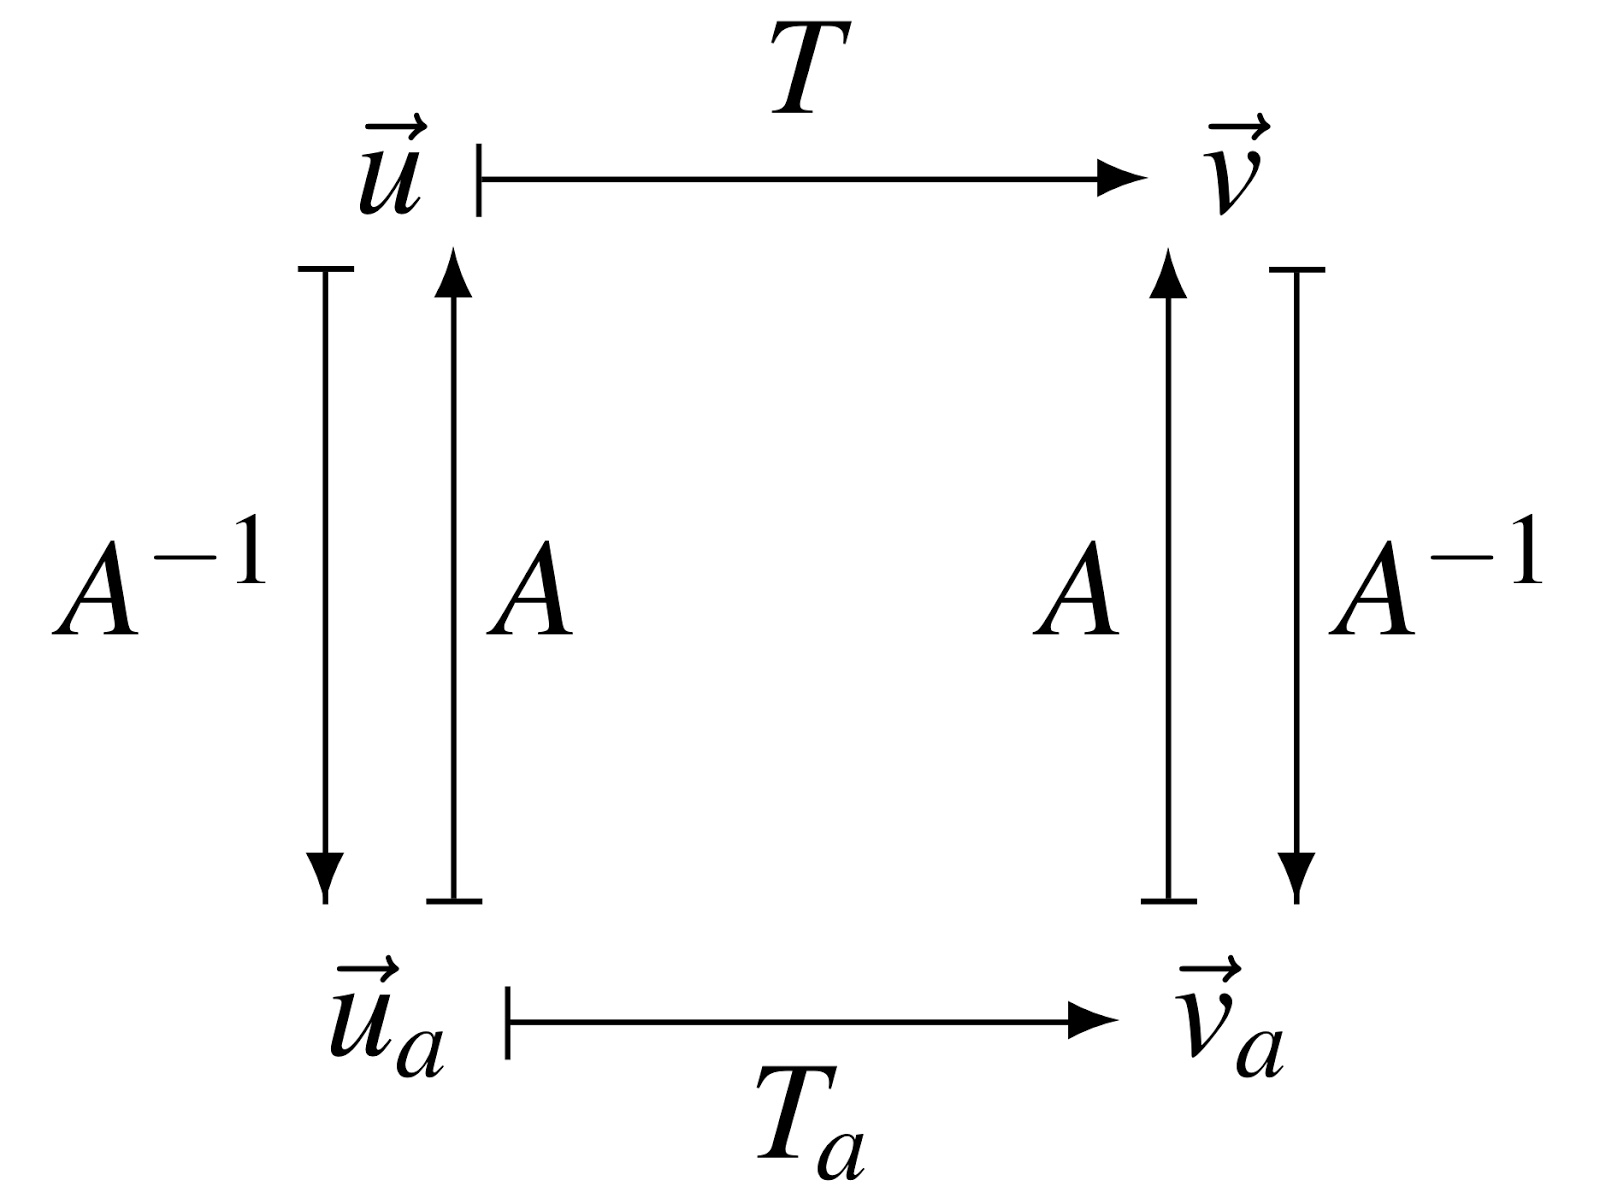
\includegraphics[width=40mm]{change-of-basis-diagram.jpeg}
	    \end{columns}
	\end{frame}
	
	\begin{frame}{Diagonalization}
	    \begin{itemize}
	        \item The idea is that we want to change into a basis in which the system $A\vec{x} = \vec{y}$ is represented by a diagonal matrix. So how do we find such basis?
	        
	        \item Remember that for all eigenvalue-eigenvector pairs we have: $A\vec{v} = \lambda\vec{v}$
	        
	        \item Let’s use our eigenvectors as our basis. Doing so we obtain:
	        
	        $$\vec{x} = V\tilde{\vec{x}}, \vec{y} = V\tilde{\vec{y}}, \text{and} \Lambda\tilde{\vec{x}} = \tilde{\vec{y}}$$
	        
	        Where the upper-case lambda represents the diagonal matrix with eigenvalues on the diagonals.
	        
	        \item Transforming back to the standard basis, we get:
            
            $$A = V\Lambda{V^{-1}}$$
	    \end{itemize}
	\end{frame}
	
	\begin{frame}{Diagonalization Cont.}
	    \begin{itemize}
	        \item Let’s analyze this a bit further, why is it important to be able to do this?
            
            \item We see that diagonalizing the matrix makes the system much easier to solve, why? 
            
            \item Also, we see that there is a “home state” for every system of linearly independent equations, i.e. the space in which the system’s components are uncoupled.
	    \end{itemize}
	\end{frame}
	
	\begin{frame}
	    2 min break
	\end{frame}
	
	\begin{frame}{Solving Differential Equations}
	    Differentiation is linear!
	    
	    $$\frac{d(c_1x(t) + c_2y(t))}{dt} = c_1\frac{dx(t)}{dt} + c_2\frac{dy(t)}{dt}$$
	\end{frame}
	
	\begin{frame}{Solving systems of differential equations}
	    Write the system in the following form:

        $$\frac{dx(t)}{dt} = Ax(t)$$
        
        Find the eigenvalues/eigenvectors of $A$ and transform the system into the eigenbasis. If $A$ has distinct eigenvalues, the general solution is:
        
        $$x(t) = c_1e^{\lambda_1{t}}\vec{v_1} + c_2e^{\lambda_2{t}}\vec{v_2}$$
        
        Then, change back to the standard basis.
	\end{frame}
	
	\begin{frame}{Example: second-order differential equations}
	    Solve the following differential equation:

        $$\ddot{x} - \dot{x} - 2x = 0$$
        
        $$x(0) = 2, \dot{x}(0) = 1$$
	\end{frame}
	
	\begin{frame}{Example: second-order differential equations}
	    $\ddot{x} - \dot{x} - 2x = 0$, $x(0) = 2, \dot{x}(0) = 1$
	    
	    Solution:
	    
	    Write in matrix form and find eigenvectors:
	    $$\mat{\dot{x};\ddot{x}} = \mat{0 1; 2 1}\mat{x;\dot{x}}$$
	    
	    $$\lambda_1 = 2, v_1 = \mat{1;2}, \lambda_2 = -1, v_2 = \mat{-1;1}$$
	    
	    Use general form to solve:
	    
	    $$\mat{x;\dot{x}} = c_1e^{2t}v_1 + c_2e^{-t}v_2$$
	\end{frame}
	
	\begin{frame}{Example: second-order differential equations}
	    $\ddot{x} - \dot{x} - 2x = 0$, $x(0) = 2, \dot{x}(0) = 1$
	    
	    Solution:
	    
	    Now plug in initial conditions:
	    $$\mat{2;1} = \mat{x(0); \dot{x}(0)} = c_1v_1 + c_2v_2 = \mat{c_1-c_2;2c_1+c_2}$$
	    
	    Solving, we get $c_1 = 1, c_2 = -1$
	    
	    so $x(t) = e^{2t} + e^{-t}$
	\end{frame}
	
	\begin{frame}{Example: second-order differential equations}
	    $\ddot{x} - \dot{x} - 2x = 0$, $x(0) = 2, \dot{x}(0) = 1$
	    
	    Solution:
	    
	    Sanity check: compute derivatives and check that the original system is satisfied
	    
	    $x(t) = e^{2t} + e^{-t}, \dot{x}(t) = 2e^{2t} - e^{-t}, \ddot{x}(t) = 4e^{2t} + e^{-t}$
	    
	    $\implies \ddot{x} - \dot{x} - 2x = 0, x(0) = 2, \dot{x}(0) = 1$
	\end{frame}
	
	\begin{frame}{Example: second-order differential equations}
	    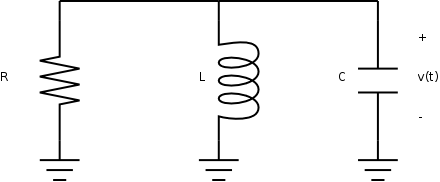
\includegraphics[width=0.6\textwidth]{second-order-1.png}
	    
	    Given $x(t) = \mat{v(t);i_L(t)}$
	    
	    find matrix $A$ such that $\frac{dx}{dt} = Ax$
	\end{frame}
	
	\begin{frame}{Example: second-order differential equations}
    	\begin{columns}[onlytextwidth,T]
        	\column{\dimexpr\linewidth-40mm-5mm}
        	Direct all currents into ground.
	        
	        $$i_R + i_L + i_C = 0$$
	        
	        $$\frac{V}{R} + i_L = -C\frac{dV}{dt}$$
	        
	        $$-\frac{1}{CR}V + -\frac{1}{C}i_L = \frac{dV}{dt}$$
	        
	        Also $L\frac{di_L}{dt} = V \implies A = \mat{-\frac{1}{RC} -\frac{1}{C}; \frac{1}{L} 0}$
	        
	        \column{40mm}
	        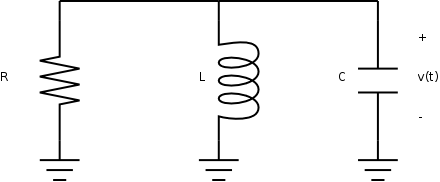
\includegraphics[width=40mm]{second-order-1.png}
        \end{columns}
	\end{frame}
	
	\begin{frame}{Example: second-order differential equations}
	    \begin{columns}[onlytextwidth,T]
        	\column{\dimexpr\linewidth-40mm-5mm}
        	    At $t < 0$, the circuit is at steady state. At $t \geq 0$, the voltage source is set to 0. Find a differential equation for $i_L$ for $t \geq 0$.
        	
        	\column{40mm}
        	    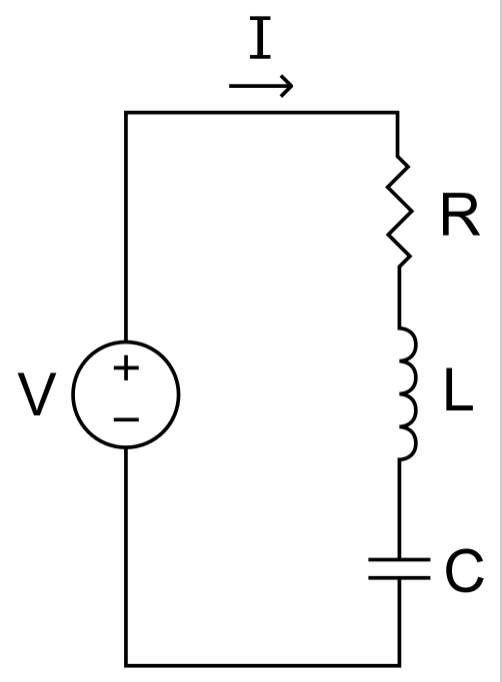
\includegraphics[width=40mm]{second-order-2.png}
    	\end{columns}
	\end{frame}
	
	\begin{frame}{Example: second-order differential equations}
	    \begin{columns}[onlytextwidth,T]
        	\column{\dimexpr\linewidth-40mm-5mm}
        	    Solution: use KCL/KVL to get
        	    
        	    $$i_R = i_L = i_C, V_C + V_R + V_L = 0$$
        	    
        	    $$\frac{V_R}{R} = i_L = C\frac{dV_C}{dt}, \frac{1}{C}i_L + R\frac{di_L}{dt} + L\frac{d^2i_L}{dt} = 0$$
        	    
        	    $$\mat{\frac{di_L}{dt}; \frac{d^2i_L}{dt}} = \mat{0 1; -\frac{1}{LC} -\frac{R}{L}}\mat{i_L;\frac{di_L}{dt}}$$
        	    
        	\column{40mm}
        	    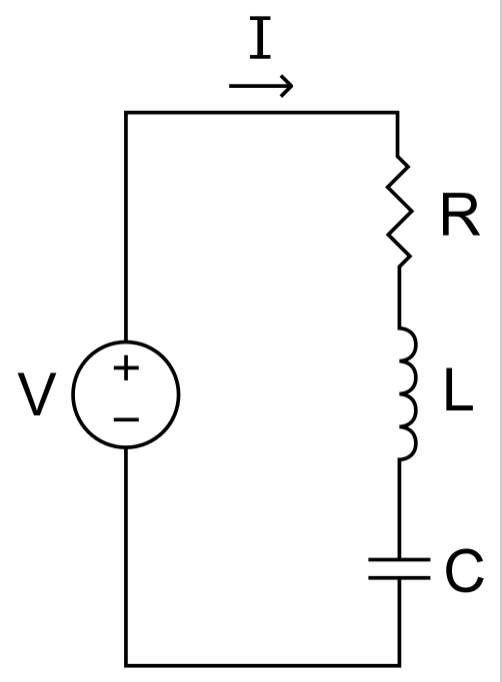
\includegraphics[width=40mm]{second-order-2.png}
    	\end{columns}
	\end{frame}
	
	\begin{frame}{Example: second-order differential equations}
	    \begin{columns}[onlytextwidth,T]
        	\column{\dimexpr\linewidth-40mm-5mm}
        	    If $R = 0$, $L = C = 1$, solve the differential equation:
        	    
        	    Initial conditions: $i_L(0) = 0$, $\frac{di_L}{dt}(0) = -V_c = -V$
        	    
        	    Differential equation: $\mat{\frac{di_L}{dt}; \frac{d^2i_L}{dt}} = \mat{0 1; -\frac{1}{LC} -\frac{R}{L}}\mat{i_L;\frac{di_L}{dt}}$
        	    
        	    $$\lambda_1 = i, v_1 = \mat{i;-1}$$
        	    
        	    $$\lambda_2 = -i, v_2 = \mat{i;1}$$
        	    
        	\column{40mm}
        	    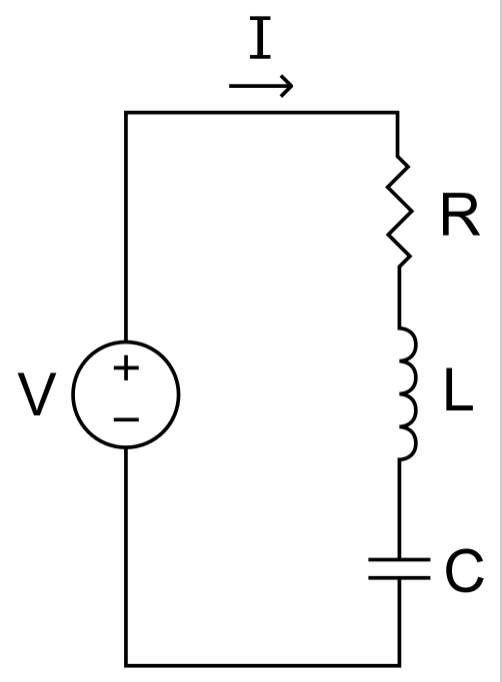
\includegraphics[width=40mm]{second-order-2.png}
    	\end{columns}
	\end{frame}
	
	\begin{frame}{Example: second-order differential equations}
	    \begin{columns}[onlytextwidth,T]
        	\column{\dimexpr\linewidth-40mm-5mm}
        	    $$\mat{i_L;\frac{di_L}{dt}} = c_1e^{it}v_1 + c_2e^{-it}v_2$$
        	    
        	    $$ic_1 + ic_2 = 0, -c_1 + c_2 = -V$$
        	    
        	    $$\implies c_1 = \frac{V}{2}, c_2 = -\frac{V}{2}$$
        	    
        	    so
        	    
        	    $$i_L = \frac{V}{2}ie^{it} - \frac{V}{2}e^{-it}$$
        	    
        	\column{40mm}
        	    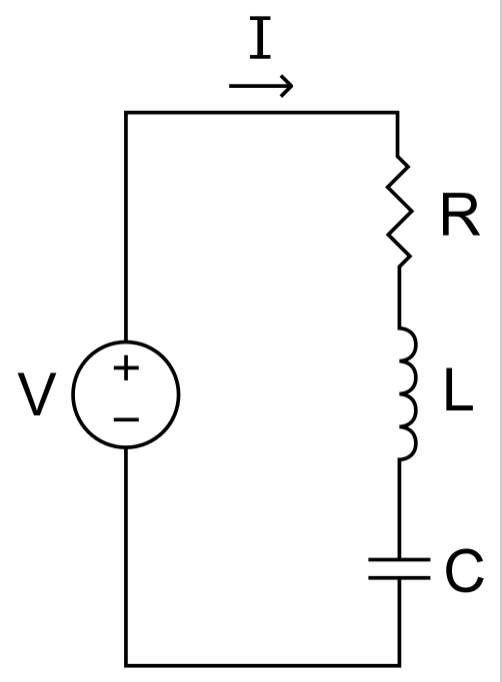
\includegraphics[width=40mm]{second-order-2.png}
    	\end{columns}
	\end{frame}
	
	\begin{frame}{Example: 2 coupled diff eqs}
	    Consider a system of 2 coupled harmonic oscillators, described by

        $$m_i\ddot{x}_i = -(k + \kappa)x_i + \kappa{}x_j$$
        
        \begin{center}
            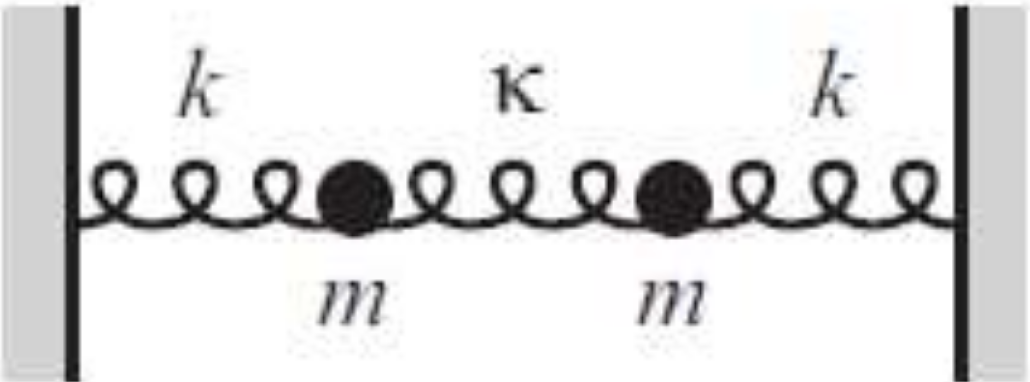
\includegraphics[width=0.5\textwidth]{coupled-eq-1.png}
        \end{center}
	\end{frame}
	
	\begin{frame}{Example: Coupled Oscillator}
	    Write this system in matrix form
        
        $$m_i\ddot{x}_i = -(k + \kappa)x_i + \kappa{}x_j$$
	\end{frame}
	
	\begin{frame}{Example: Coupled Oscillator}
	    Write this system in matrix form
        
        $$m_i\ddot{x}_i = -(k + \kappa)x_i + \kappa{}x_j$$
        
        \begin{center}
         \scalebox{2}{$\ddot{\vec{x}} = \mat{-\frac{k+\kappa}{m} \frac{\kappa}{m}; \frac{\kappa}{m} -\frac{k+\kappa}{m}}\vec{x}$}
        \end{center}
	\end{frame}
	
	\begin{frame}{Example: Coupled Oscillator}
	    Now, diagonalize the system

	    \begin{center}
         \scalebox{2}{$\mat{-\frac{k+\kappa}{m} \frac{\kappa}{m}; \frac{\kappa}{m} -\frac{k+\kappa}{m}} = PDP^{'}$}
        \end{center}
        
        P = ?
        
        D = ?
	\end{frame}
	
	\begin{frame}{Example: Coupled Oscillator}
	    Now, diagonalize the system

	    \begin{center}
         \scalebox{2}{$\mat{-\frac{k+\kappa}{m} \frac{\kappa}{m}; \frac{\kappa}{m} -\frac{k+\kappa}{m}} = PDP^{'}$}
        \end{center}
        
        $$P = \mat{1 1; 1 -1}$$
        
        $$D = \mat{k 0; 0 2\kappa+k}$$
	\end{frame}
	
	\begin{frame}{Example: Coupled Oscillator}
	    $$P = \mat{1 1; 1 -1}$$
        
        $$D = \mat{k 0; 0 2\kappa+k}$$
        
        Since our original matrix was linearly taking a SECOND derivative in time, with only real eigenvalues, we expect solutions to be in the form of real sinusoids, optionally phaseshifted.

        $$x(t) = A_s\mat{1;1}\cos(\sqrt{\frac{k}{m}}t + \phi_s) + A_f\mat{1;-1}\sin(\sqrt{\frac{k + 2\kappa}{m}}t + \phi_f)$$
	\end{frame}
	
	\begin{frame}{What do we do with different types of eigenvalues?}
	    Each interesting “case” of eigenvalues (real, imaginary, and repeated) is complementary to a case of resonance in 2d ODEs, so let’s discuss them together:
        
        \begin{center}
            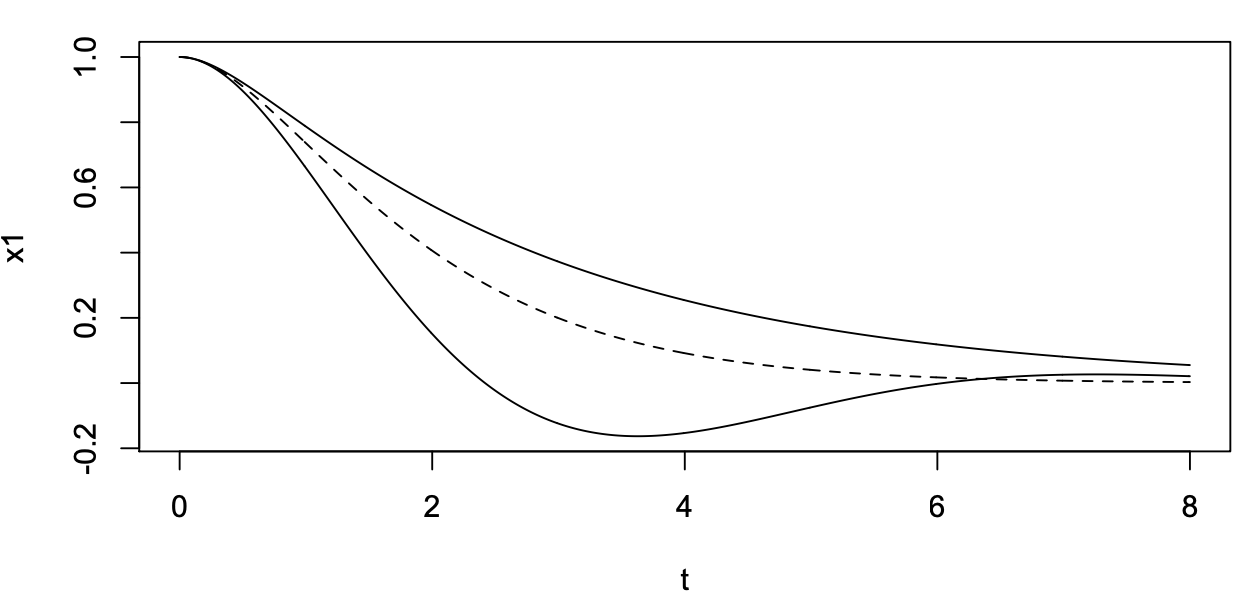
\includegraphics[width=0.5\textwidth]{eigenvalue-types-1.png}
        \end{center}
	\end{frame}
	
	\begin{frame}{Overdamping: two real eigenvalues}
	    \begin{itemize}
	        \item When a system has two real eigenvalues, it will have two real eigenvectors, so the solution will be a combination of exponentials in the form 
            
            $$ae^{\lambda_1t} + be^{\lambda_2t}$$
            
            \item For negative lambdas, this produces exponential decay.
            
            \item
            \begin{columns}[onlytextwidth,T]
            \column{\dimexpr\linewidth-40mm-5mm}
        	    At large t, greater eigenvalue dominates behavior, so how fast the system approaches to 0 is determined by the larger eigenvalue.
        	
        	\column{40mm}
        	    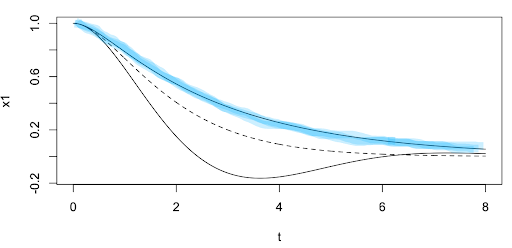
\includegraphics[width=40mm]{eigenvalue-types-3.png}
    	    \end{columns}
	    \end{itemize}
	\end{frame}
	
	\begin{frame}{Underdamping: imaginary or complex eigenvalues}
	    \begin{itemize}
	        \item You can still solve the system of differential equations as usual, but your solutions will be complex:
            
            $$(a_1j + b_1)e^{c_1j + d_1} + (a_2j + b_2)e^{c_2j + d_2}$$
            
            \item You can rearrange terms and apply Euler’s formula to write each term as a real exponential multiplied by a sinusoid
            $$e^{d_1}(\alpha_1sin(...) + \beta_1cos(...)) + e^{d_2}(\alpha_2sin(...) + \beta_2cos(...))$$
            
            \item
            \begin{columns}[onlytextwidth,T]
            \column{\dimexpr\linewidth-40mm-5mm}
        	    If $d_1$ and $d_2$ are negative, then you can think of this as a sinusoid where the amplitude decays to 0
        	
        	\column{40mm}
        	    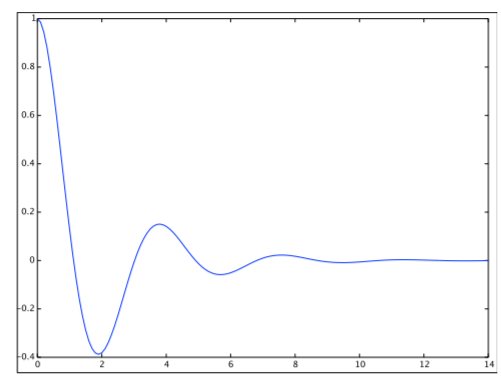
\includegraphics[width=40mm]{eigenvalue-types-2.png}
    	    \end{columns}
	    \end{itemize}
	\end{frame}
	
	\begin{frame}{Critical Damping: repeated eigenvalue}
	    \begin{itemize}
	        \item You only get one linearly independent eigenvector. 
            
            \item So, arbitrarily choose the second column of your $V$ matrix (making sure it is linearly independent from the eigenvector $v_1$)
            
            \item Compute $A_v$ using the change of basis diagram $A_v = V^{-1}AV$
            
            \item This gives you an upper-triangular matrix
            
            \item The bottom row of the matrix gives you an equation in one variable (only depends on the second component of $x_v$), which you can solve to get something in the form of $x_{v,2} = ae^{\lambda{t}}$
	    \end{itemize}
	\end{frame}
	
	\begin{frame}{Critical Damping: repeated eigenvalue}
	    \begin{itemize}
	        \item The top row of the matrix depends on both components of $x_v$, but you can plug in the value you got for $x_{v,2}$ and then solve for $x_{v,1}$
            
            \item If you solve this differential equation (which is a diff eq with a non-constant input*), you’ll get an equation in the form:
            
            $$x(t) = c_1e^{-\lambda{t}} + c_2te^{-\lambda{t}}$$
            
            \item
            \begin{columns}[onlytextwidth,T]
            \column{\dimexpr\linewidth-40mm-5mm}
        	    \textbf{The critically damped case gives us the fastest-decaying exponential that doesn’t oscillate}
        	
        	\column{40mm}
        	    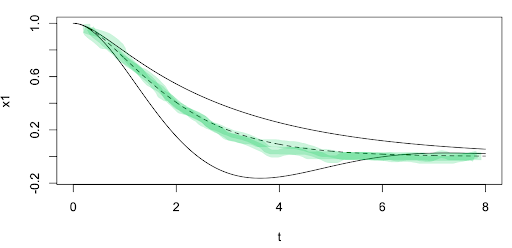
\includegraphics[width=40mm]{eigenvalue-types-4.png}
    	    \end{columns}
	    \end{itemize}
	    
	    *You can solve this using the formula $x_p(t) = x_0e^{\lambda{t}} + \int_0^t u(\tau)e^{\lambda(t-\tau)} d\tau$
	\end{frame}
	
	\begin{frame}
	    2 min break
	\end{frame}
	
	\section{Phasors}
	
    \begin{frame}{Phasors}
        \begin{itemize}
            \item Phasors express the response of a circuit to a sinusoidal input
            \item Any real, periodic signal can be expresses as the sum of sinusoids - we can apply this technique very broadly!
            \item A phasor encodes information about amplitude and phase, but not frequency
            $$v_s=A\cos(\omega t+\phi) \rightarrow \tilde{V}_s=Ae^{j\phi}$$
        \end{itemize}
    \end{frame}
    
    \begin{frame}{Impedance}
        \begin{itemize}
            \item Impedance ($Z$) is a generalized form of resistance - expresses a component's response to an alternating current
            \item Each common passive circuit element (resistor, capacitor, and inductor) has a characteristic impedance
            $$Z_R=R$$
            $$Z_C=\frac{1}{j\omega C}$$
            $$Z_L=j\omega L$$
        \end{itemize}
    \end{frame}
    
    \begin{frame}{Phasor Analysis Procedure}
        \begin{enumerate}
            \item Express all time domain signals as cosines
            \item Convert voltages, currents, and impedances to their phasor equivalents
            \item Set up phasor equations and solve for unknowns
            \item Transform back to time domain
        \end{enumerate}
    \end{frame}
    
    \begin{frame}{Phasor Practice}
        \begin{center}
            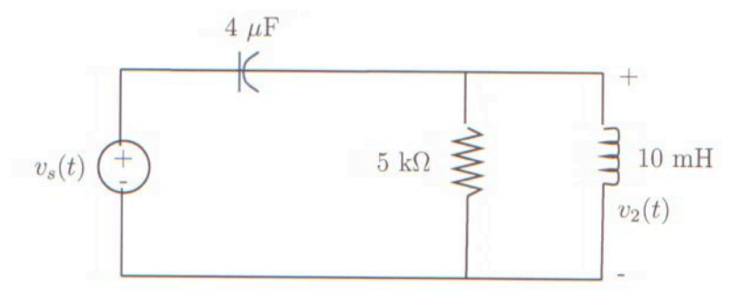
\includegraphics[width=0.5\textwidth]{phasor-practice.png}
        \end{center}
        Let $v_s(t)=5\cos(5000t+\frac{\pi}{4})$. Find $v_2(t)$.
    \end{frame}

    \begin{frame}{Phasor Practice}
        \begin{center}
            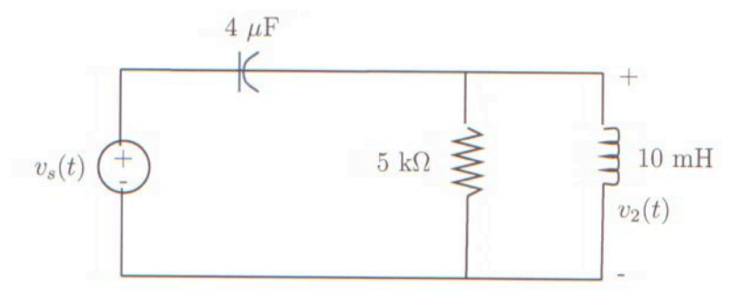
\includegraphics[width=0.5\textwidth]{phasor-practice.png}
        \end{center}
        \begin{enumerate}
            \item Translate to phasor domain
            \begin{itemize}
                \item $\omega=5000$
                \item $v_s(t)=5\cos(5000t+\frac{\pi}{4})\rightarrow \tilde{V}_s=5e^{j\frac{\pi}{4}}$
                \item $C=4\mu F\rightarrow Z_C=\frac{1}{j(4*10^{-6})(5000)}=-j50$
                \item $R=5k\Omega\rightarrow Z_R=5*10^3$
                \item $L=10mH\rightarrow Z_L=j(5000)(10*10^{-3})=j50$
            \end{itemize}
        \end{enumerate}
    \end{frame}
    
    \begin{frame}{Phasor Practice}
        \begin{center}
            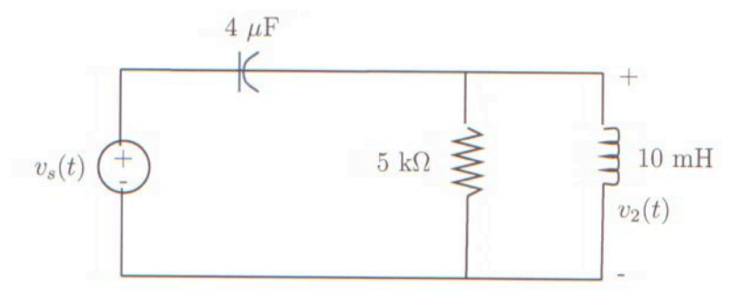
\includegraphics[width=0.5\textwidth]{phasor-practice.png}
        \end{center}
        \begin{enumerate}
            \item[2.] Solve for $\tilde{V}_2$
            \begin{itemize}
                \item Set up as impedance divider: $$\frac{\tilde{V}_s}{Z_C+(Z_R\| Z_L)}=\frac{\tilde{V}_2}{Z_R\| Z_L}$$
                $$\tilde{V}_2=\tilde{V}_s\frac{Z_R\|Z_L}{Z_C+(Z_R\|Z_L)}=\tilde{V}_s\frac{\frac{Z_RZ_L}{Z_R+Z_L}}{\frac{Z_RZ_L+Z_RZ_C+Z_LZ_C}{Z_R+Z_L}}$$
            \end{itemize}
        \end{enumerate}
    \end{frame}
    
    \begin{frame}{Phasor Practice}
        \begin{center}
            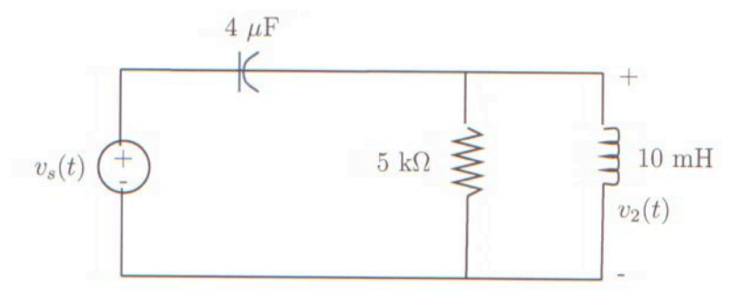
\includegraphics[width=0.5\textwidth]{phasor-practice.png}
        \end{center}
        \begin{enumerate}
            \item[2.] Solve for $\tilde{V}_2$
            $$\tilde{V}_2=\tilde{V}_s\frac{Z_RZ_L}{Z_RZ_L+Z_RZ_C+Z_LZ_C}=\tilde{V}_s\frac{j2.5*10^5}{j2.5*10^5-j2.5*10^5+2500}$$
            $$\tilde{V}_2=j100\tilde{V}_s=100\tilde{V}_se^{j\frac{\pi}{2}}$$
        \end{enumerate}
    \end{frame}
    
    \begin{frame}{Phasor Practice}
        \begin{center}
            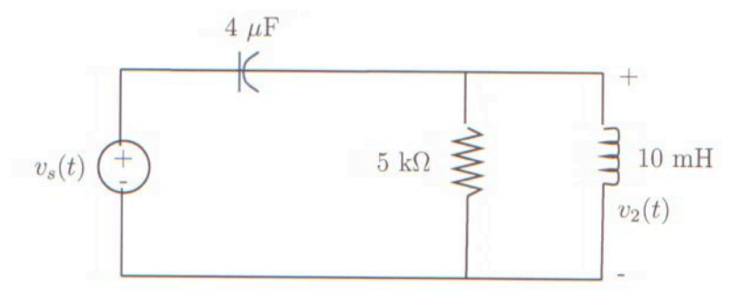
\includegraphics[width=0.5\textwidth]{phasor-practice.png}
        \end{center}
        \begin{enumerate}
            \item[3.] Find time-domain solution
            \begin{itemize}
                \item $\tilde{V}_2=100e^{j\frac{\pi}{2}}\tilde{V}_s\rightarrow v_2(t)=100v_s(t+\frac{\pi}{2})=500\cos(5000t+\frac{3\pi}{4})$
            \end{itemize}
        \end{enumerate}
    \end{frame}
	
%This should be slides 69-86
    \begin{frame}{Transfer Function Review}
        A \textbf{\emph{transfer function}} of a circuit or system describes the \textcolor{red}{output response} to an \textcolor{red}{input excitation} as a function of the angular frequency $\omega$.
        \begin{center}
            $H(\omega) = \frac{V_{out}(\omega)}{V_{in}(\omega)}$
        \end{center}
    \end{frame}
    \begin{frame}{RC Circuits}
        \begin{columns}
            \begin{column}{0.5\textwidth}
            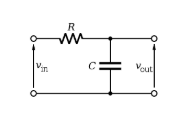
\includegraphics[]{rc-circuits_1.png}\\ \\
                $H(\omega) = \frac{1}{1 + j\omega RC}$\\ \\
                \textbf{Low pass:} $\lim_{\omega\to\infty} H(\omega) = 0, H(0) = 1$
                
            \end{column}
            \begin{column}{0.5\textwidth}
            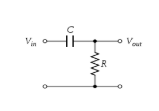
\includegraphics[]{rc-circuits_2.png} \\ \\ 
                $H(\omega) = \frac{j\omega RC}{1 + j\omega RC}$\\ \\
                \textbf{High pass:} $\lim_{\omega\to\infty} H(\omega) = 1, H(0) = 0$
            \end{column}
            
        \end{columns}
    \end{frame}
    
    \begin{frame}{Bode Plot Review}
        $V[dB] = 20\log_{10}(\frac{V}{V_0})$
        \begin{itemize}
            \item Bode plots provide a way for us to easily visualize the output response of our system, depending on the input frequency $\omega$. 
            \item Because Bode plots are in log scale for $\omega$, we are able to take advantage of the properties of logs.
            \begin{itemize}
                \item $G = XY \implies G[dB] = X[dB] + Y[dB]$
                \item $G = \frac{X}{Y} \implies G[dB] = X[dB] - Y[dB]$
            \end{itemize}
        \end{itemize}
        Hence, we can break our transfer function H($\omega$) into a product of familiar transfer functions (simple poles, quadratic zeros, etc. - “functional forms”), graph them out individually, and then add them together on the graph.  
    \end{frame}
    \begin{frame}{Bode Plot Review}
        \begin{itemize}
            \item We want to be able to plot the transfer function as a function of the frequency $\omega$. 
            \item However, it’s a complex valued function so it’s easier to have a plot for the magnitude and one for the phase. 
            \item Because the magnitude plot is in log scale, and the phase plot is in semi-log scale we are able to take advantage of the properties of logs. 
            \begin{itemize}
                \item $\log(XY) = \log(X) + \log(Y)$
            \end{itemize}
            \item Hence, we can break our transfer function H($\omega$) into a product of familiar transfer functions (simple poles, quadratic zeros, etc. - “functional forms”), graph them out individually, and then add them together on the graph.
        \end{itemize}
    \end{frame}
    \begin{frame}{Bode Plot Steps}
        \begin{enumerate}
            \item Break transfer function into product of functional forms
            \begin{enumerate}
                \item $H(\omega) = \frac{n(\omega)}{d(\omega)} = \frac{(j\omega)^n\alpha_{n} + (j\omega)^{n-1}\alpha_{n-1} + \ldots  + j \omega \alpha_1 + \alpha_0}{(j\omega)^n\beta_{n} + (j\omega)^{n-1}\beta_{n-1} + \ldots  + j \omega \beta_1 + \beta_0} = \kappa \frac{(j\frac{\omega}{\omega_{z1}} +1)(j\frac{\omega}{\omega_{z2}} +1) \ldots}{(j\frac{\omega}{\omega_{\rho1}} +1)(j\frac{\omega}{\omega_{\rho2}} +1) \ldots}$
            \end{enumerate}
            \item Graph each transfer function individually
            \item Add them up on the graph (thanks to log scale)
            \begin{enumerate}
                \item 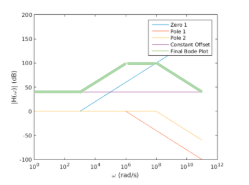
\includegraphics[scale=0.5]{bode-plot-steps-1.png}
            \end{enumerate}
        \end{enumerate}
    \end{frame}
    \begin{frame}{RC Circuits, revisited}
        \begin{columns}
            \begin{column}{0.5\textwidth}
                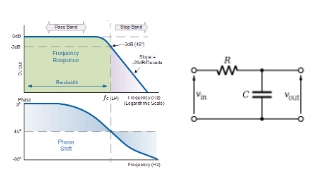
\includegraphics[scale=0.75]{Rc-circuits-revisited-1.png}\\
                $H(\omega) = \frac{1}{1 + j\omega RC}$
            \end{column}
            \begin{column}{0.5\textwidth}
                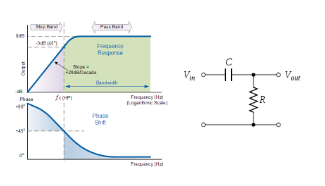
\includegraphics[scale=0.75]{rc-circuits-revisited-2.png}\\
                $H(\omega) = \frac{j\omega RC}{1 + j\omega RC}$
            \end{column}
            
        \end{columns}
    \end{frame}
    \begin{frame}{Important Functional Forms}
        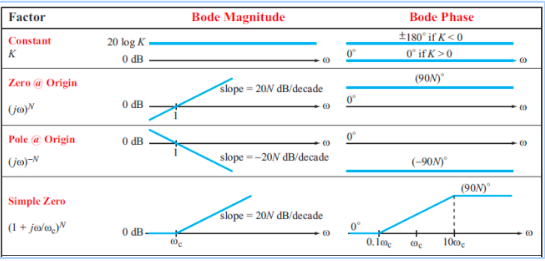
\includegraphics[scale=0.75]{important-functional-forms-1.png}
    \end{frame}
    \begin{frame}{Important Functional Forms}
        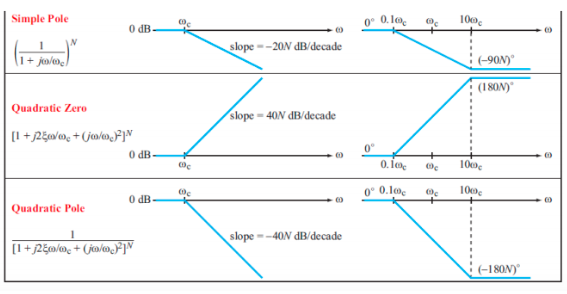
\includegraphics[scale=0.75]{important-functional-forms-2.png}
    \end{frame}
    \begin{frame}{Practice Problem}
        $$H(\omega) = \frac{\frac{j\omega}{10} + 100}{1 + \frac{(j\omega)^2}{10^14} + \frac{j\omega}{10^8} + \frac{j\omega}{10^6}}$$\\
        \begin{center}
            Draw the Bode plot for this transfer function.
        \end{center}
    \end{frame}
    \begin{frame}{}
        \begin{columns}
            \begin{column}{0.5\textwidth}
                $$H(\omega) = \frac{\frac{j\omega}{10} + 100}{1 + \frac{(j\omega)^2}{10^14} + \frac{j\omega}{10^8} + \frac{j\omega}{10^6}}$$\\
                $$=\frac{100(\frac{j\omega}{10^3}+1)}{(\frac{j\omega}{10^6}+1)(\frac{j\omega}{10^8}+1)}
                $$
            \end{column}
            \begin{column}{0.5\textwidth}
                Main idea: break our transfer function into the product of standard forms- a constant, one zero, and two poles
            \end{column}
        \end{columns}
        
    \end{frame}
    \begin{frame}{}
        \begin{columns}
            \begin{column}{0.25\textwidth}
                Final Result
            \end{column}
            \begin{column}{0.75\textwidth}
                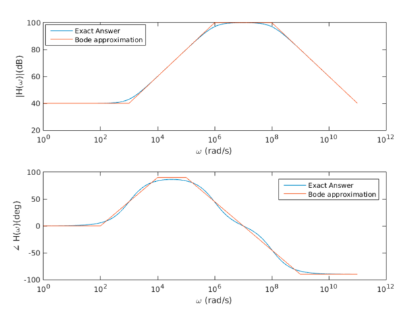
\includegraphics[scale=0.75]{practice-problem.png}\\
            \end{column}
        \end{columns}
    \end{frame}
    \begin{frame}{Common Filters and their Bode Plots}
        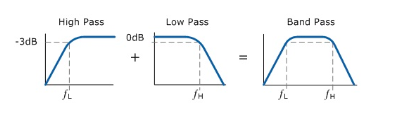
\includegraphics[]{common-filter-bode-plot.png}\\
        In the high pass filter, the frequencies greater than the corner frequency have a gain of 0dB (so they aren’t changed), while frequencies less than the corner frequency have a gain < 0dB (so they are multiplied by something less than 1). \\
        In the lowpass filter, the opposite is true.
    \end{frame}
    \begin{frame}{Design Problem}
        Design an active high pass filter with cutoff frequency of 1KHz and a gain of 1000.\\
        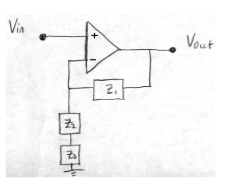
\includegraphics[scale=0.65]{design-problem-summary.png}\\
        \begin{itemize}
            \item Hint 1:  Find the transfer function of the following circuit.
            \item Hint 2: Which transfer function is a high pass filter?
            \begin{itemize}
                \item $H_1(\omega) = 1 + \frac{j\omega R_1C}{1 + j\omega R_2C}$
                \item $H_2(\omega) = 1 + \frac{R_1R_2}{1 + j\omega R_1C}$
            \end{itemize}
            \item Hint 3: What is the impedance of a resistor in series with a capacitor?
            \item Hint 4: Replace the Z’s with resistors/capacitors/wires/open circuits.
        \end{itemize}
    \end{frame}
    \begin{frame}{Design Problem: Hint 1}
        \begin{itemize}
            \item Step 1: Apply the golden rules of Op. Amps. This means that $V^+ = V^-$.
            \item Step 2: By ohm’s law, we can calculate the current from V- to ground.
            \begin{itemize}
                \item $I = \frac{V_{in}}{Z_2 + Z_3}$
            \end{itemize}
            \item Step 3: By Ohm’s law, we can calculate the output voltage.
            \begin{itemize}
                \item $V_{out} = V_{in}(1 + \frac{Z_1}{Z_2 + Z_3})$
            \end{itemize}
        \end{itemize}
    \end{frame}
    \begin{frame}{Design Problem: Hint 2 + Hint 3}
        \begin{itemize}
            \item The high pass filter transfer function is: $H_1(\omega) = 1 + \frac{j\omega R_1C}{1 + j\omega R_2C}$
            \item To more easily separate the gain from the frequency filtering, we can approximate it as (at high frequencies): $H_1(\omega) = \frac{R_1}{R_2}(\frac{j\omega R_2C}{1 + j\omega R_2 C})$
            \item A resistor in series with a capacitor has impedances of: $R + \frac{1}{j\omega C} = \frac{j \omega RC +1}{j\omega C}$
        \end{itemize}
    \end{frame}
    \begin{frame}{Design Problem: Summary of Hints}
    Now, use all of the earlier hints to get a high pass filter!\\
    (Cutoff Frequency is 1KHz, gain of 1000)\\
    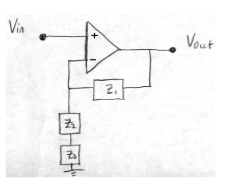
\includegraphics[scale=0.75]{design-problem-summary.png}\\
    $V_{out} = V_{in}(1 + \frac{Z_1}{Z_2+Z_3})$\\
    $H_1(\omega) = 1 + \frac{j\omega R_1 C}{1 + j \omega R_2 C}$ \\
    $R + \frac{1}{j\omega C} = \frac{j \omega RC + 1}{j \omega C}$
    \end{frame}
    \begin{frame}{Design Problem Solution}
        We implement the circuit such that it has the transfer function of :\\
        $$H_1(\omega) = 1 + \frac{j\omega R_1C}{1 + j\omega R_2C}$$\\
        To meet our specifications: \\
        $$\frac{R_1}{R_2} = 1000$$ \\
        $$R_2C = \frac{1}{2\pi(1000)}$$\\
        One Possible Solution: \\
        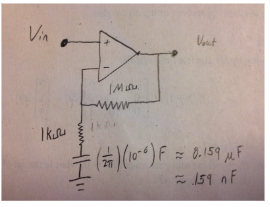
\includegraphics[scale=0.65]{design-problem-solution.png}
    \end{frame}
    \begin{frame}{}
        \begin{center}
            Good luck on your midterm!\\
            Feedback Form: hkn.mu/feedback\\
            
\includegraphics[]{dog.png}
        \end{center}
        
    \end{frame}

    
\end{document}